\subsection{Closed Loop}
\label{sec:closed_loop}
\begin{figure*}
\centering
%\vspace*{-0.3cm}  
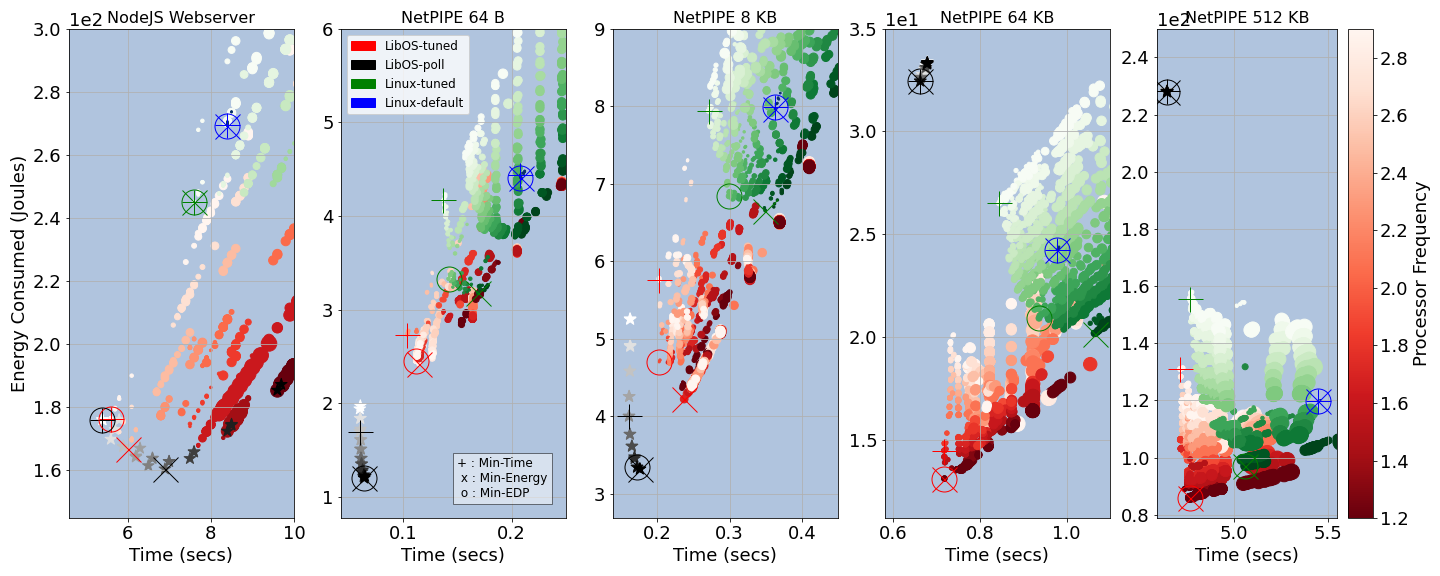
\includegraphics[width=1\textwidth]{figures/closed_loop_overview.png}
\caption[]
%{\small 
{Closed loops.}
\label{fig:closed_loop_overview}
\end{figure*}
\begin{figure*}
\centering
%\vspace*{-0.3cm}  
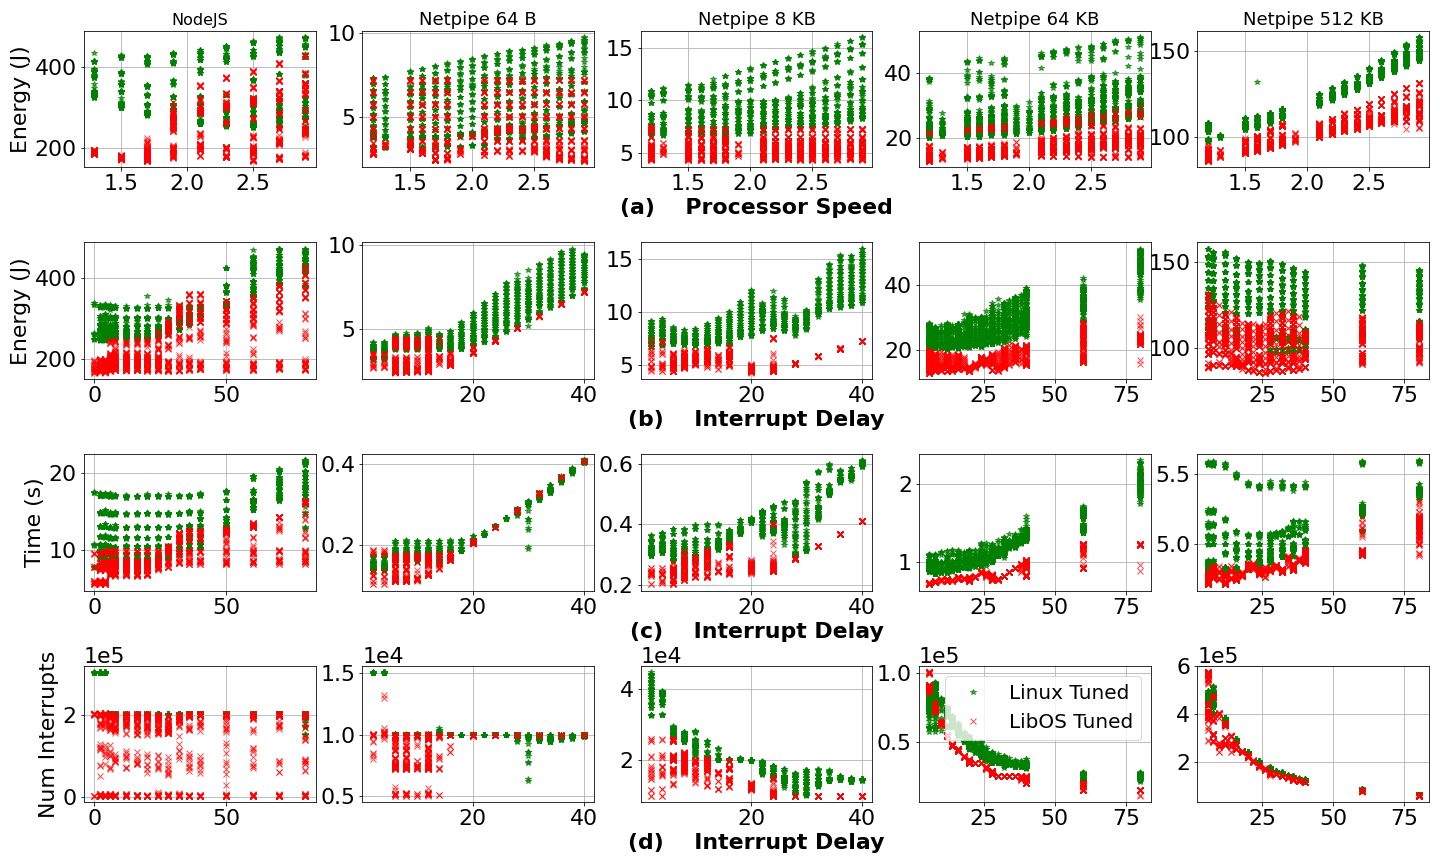
\includegraphics[width=1\textwidth]{figures/closed_detail_1.png}
\caption[]
%{\small 
{Closed loops.}
\label{fig:closed_loop_detail_1}
\end{figure*}
%This approach makes the workloads more predictable and can help smooth out diurnal variations as well~\cite{10.1145/2168836.2168842, 10.1145/2000064.2019527, oldi-study}.
% As pointed out in previous studies of energy proportionality in datacenters, the nature of web-centric applications causes diurnal troughs~\cite{Barroso:2009:DCI:1643608, oldi-study, oldi-pegasus, warehouse-power, energyproportion, WebSearch} and one method with which to increase energy efficiency during these troughs is to maximize the amount of work done, typically under a given energy budget. Figure~\ref{fig:closed_loop_overview} illustrates the set of closed-loop workloads studied in our work, all of the workloads are run in a single core with a single connection, further, they enable us to explore these simple closed-loop examples in detail in settings of computationally intensive (nodejs) and across varying network bandwidth requirements (netpipe). 

Figure~\ref{fig:closed_loop_overview} illustrates the set of closed-loop workloads studied in our work, all of the workloads are run in a single core with a single connection. Netpipe~\cite{snell1996netpipe} involves sending messages of identical size between two systems for a fixed number of iterations. We fix the iteration count at 5000 and show results for a range of message sizes. \footnote{We found that the 10 GB link is close to saturation when a message of size greater 700 KB is exchanged.}. NodeJS~\cite{nodejs} runs a JavaScript HTTP Webserver and consists of a single client, running the \textit{wrk}~\cite{wrk} benchmark\footnote{We modified \textit{wrk} to place a fixed request load of 100K.}, that sends web requests to a server thread for a fixed period of time. The server responds to each request with a small static payload of size 148 bytes. The library OS was ported to support baremetal NodeJS by providing OS interfaces that link with the V8~\cite{v8} JavaScript engine and libuv~\cite{libuv}. 

%We believe these set of workloads will help to simplify the complexity which to compare and contrast the effects of slowing down in the four types of systems listed above.

%\subsubsection{Observation-1: Computationally heavy applications exhibits more performance-energy trade-offs}
%Comparing the nodejs and netpipe workloads in figure~\ref{fig:closed_loop_overview}, one can see the differences in trade-offs as processor is slowed. In netpipe, the \textit{vertical-ness} as the datapoints get darker shows that slowing down the processor does not cause an increase in time, whereas the opposite is shown in the nodejs data.

% MIN-TIME linux_default 1 3.0 8.396 269.4
% MIN-TIME linux_tuned 2 2.9 7.599 244.93

% MIN-TIME linux_default 64 1 3.0 0.21 4.44
% MIN-TIME linux_tuned 64 2 2.9 0.14 4.17

% MIN-TIME linux_default 8192 1 3.0 0.36 7.99
% MIN-TIME linux_tuned 8192 8 2.8 0.27 7.94

% MIN-TIME linux_default 65536 1 3.0 0.98 24.25
% MIN-TIME linux_tuned 65536 8 2.9 0.84 26.5

% MIN-TIME linux_default 524288 1 3.0 5.45 119.77
% MIN-TIME linux_tuned 524288 8 2.9 4.77 155.56





% MIN-EDP linux_default 1 3.0 8.4 269.27 2261.6
% MIN-EDP linux_tuned 2 2.9 7.6 244.93 1861.22
% MIN-EDP linux_default 64 1 3.0 0.21 4.41 0.92
% MIN-EDP linux_tuned 64 2 2.1 0.14 3.33 0.47
% MIN-EDP linux_default 8192 1 3.0 0.36 7.99 2.89
% MIN-EDP linux_tuned 8192 10 2.0 0.3 6.84 2.05
% MIN-EDP linux_default 65536 1 3.0 0.98 24.25 23.72
% MIN-EDP linux_tuned 65536 12 1.8 0.94 20.91 19.57
% MIN-EDP linux_default 524288 1 3.0 5.45 119.77 652.63
% MIN-EDP linux_tuned 524288 28 1.2 5.06 97.04 491.22


% MIN-EDP ebbrt_tuned 4 2.9 5.6 176.11 986.11
% MIN-EDP ebbrt_poll 0 2.9 5.4 175.93 949.67

% MIN-EDP ebbrt_tuned 64 6 2.9 0.11 2.45 0.27
% MIN-EDP ebbrt_poll 64 0 1.2 0.06 1.2 0.08

% MIN-EDP ebbrt_tuned 8192 2 1.9 0.2 4.7 0.95
% MIN-EDP ebbrt_poll 8192 0 1.3 0.17 3.34 0.57

% MIN-EDP ebbrt_tuned 65536 6 1.2 0.72 13.07 9.37
% MIN-EDP ebbrt_poll 65536 6 1.3 0.66 32.45 21.48

% MIN-EDP ebbrt_tuned 524288 26 1.2 4.77 85.94 409.68
% MIN-EDP ebbrt_poll 524288 6 1.5 4.65 227.86 1058.57

% find configurations in which the OS interacts with slowing down to improve both time and energy. 
\subsubsection{Speeding up to lower energy}
Figures~\ref{fig:closed_loop_detail_1}(b)(c) shows the strong correlation that minimizing the time it takes to finish the work and also results in the least amount of energy used in closed loop workloads. Figures~\ref{fig:closed_loop_detail_1}(c) demonstrates the mechanism for slowing down interrupt delays can instead be speed up (setting a low interrupt delay value) in order to increase packet processing efficiency, and therefore reduce overall time, across all the workloads and in both systems. One can also notice the wider variation in time for nodejs in figure~\ref{fig:closed_loop_detail_1}(c), this is mainly the result of greater performance-energy trade-offs that occur in a computationally bound application.

\subsubsection{Slow-to-stay-busy effect}
In the library OS, we find slowing down of the processor results in a new energy efficient state which we term \textit{slow-to-stay-busy}. In figure~\ref{fig:closed_loop_detail_1}(d), one can see that in both nodejs and netpipe 64 B, for various interrupt delay values, the number of interrupts can be lowered by up to 90\%. Upon closer examining the data, we find slowing down of the processor actually causes this decrease in number of interrupts. The reason for this behavior in the library OS can be seen in figure~\ref{fig:timeline}; the physical transmission of OS reply packets by the network driver can occur in parallel with the un-winding of the stack back to the nodejs application and then down (again) to the network receive function to check for incoming packets. It is during this un-winding code path where slowing down of the processor actually results in a slow-to-stay-busy state where by the time the un-wind has reached the network receive function (again), the response to the initial transmitted packet has already arrived, therefore the the software is able to skip another hardware interrupt in order to effectively stay busy and process this new reply packet. This scenario only occurs in the library OS due to the run-to-completion nature of its OS structure.

\subsubsection{Trade-offs in library OS polling}
To compare both performance and energy between LibOS-poll and LibOS-tuned, we can use the energy-delay-product (EDP) metric (energy x time); borrowed from the architecture community. For nodejs, LibOS-poll results in a lower EDP than LibOS-tuned by 4\%, partially this is due to nodejs' application logic already containing a polling loop to check for inbound packets. For netpipe 64B and 8KB, EDP by polling is more effective by 1.6X and 3.3X respectively. We hypothesize this is due to the smaller payload sizes, therefore getting the work done the fastest results in the lowest energy use. As payload size increases, the workload becomes more network bound, therefore polling actually results in worse EDP by up to 2X. We find at these larger payload sizes, polling only reduced time by around 10\%, however energy consumption was over 2X worse.